\documentclass{Alexandre}
\usepackage[portuguese, ruled, linesnumbered]{algorithm2e}
\usepackage{multirow}
\usepackage{multicol}
\usepackage{color}
\usepackage{diagbox}
\usepackage{setspace}
\usepackage{listings}
\usepackage{color}
\usepackage{caption}
\usepackage{mwe}
\usepackage[normalem]{ulem}
\usepackage[framemethod=tikz]{mdframed}

\definecolor{codegreen}{rgb}{0,0.6,0}
\definecolor{codegray}{rgb}{0.5,0.5,0.5}
\definecolor{codepurple}{rgb}{0.58,0,0.82}
\definecolor{backcolour}{rgb}{0.95,0.95,0.92}

\lstdefinestyle{mystyle}{
  backgroundcolor=\color{backcolour},   commentstyle=\color{codegreen},
  keywordstyle=\color{magenta},
  numberstyle=\tiny\color{codegray},
  stringstyle=\color{codepurple},
  basicstyle=\footnotesize,
  breakatwhitespace=false,         
  breaklines=true,
  captionpos=b,                   
  keepspaces=true,                 
  numbers=left,                    
  numbersep=5pt,                  
  showspaces=false,                
  showstringspaces=false,
  showtabs=false,                  
  tabsize=2
}

\setbeamertemplate{bibliography item}[triangle]

\title{Artigo}
\subtitle{A Importância da Lucidade nos Jogos Digitais Educacionais}
\author{Alexandre Mendonça Fava\inst{1}}


\institute[UDESC]{
  \newline \newline \newline
  \inst{1}
  Mestrado Acadêmico em Computação Aplicada - PPGCA
}

\date{18 Outubro de 2019}

\subject{}

\logo{

\includegraphics[scale=0.8]{Figuras/Logo-UDESC.jpg}
}

\begin{document}


\begin{frame}
  \titlepage
\end{frame}
%[Transparência 1] Bom dia, eu me chamo Alexandre, e nessa apresentação irei falar sobre o artigo que selecionei, relacionado com minha dissertação de mestrado.


\begin{frame}{AGRADECIMENTOS}

    O presente trabalho foi realizado com apoio da Coordenação de Aperfeiçoamento de Pessoal de Nível Superior - Brasil (CAPES) - Código de Financiamento 001. 

\end{frame}
%[Transparência 2] Antes de começar, como sempre, reitero aqui que o presente trabalho foi realizado com total apoio da CAPES.


\begin{frame}{PROJETO DE MESTRADO}
    \begin{center}
        Prevenção da Violência Sexual Infantil
    \end{center}
    
    \begin{figure}
        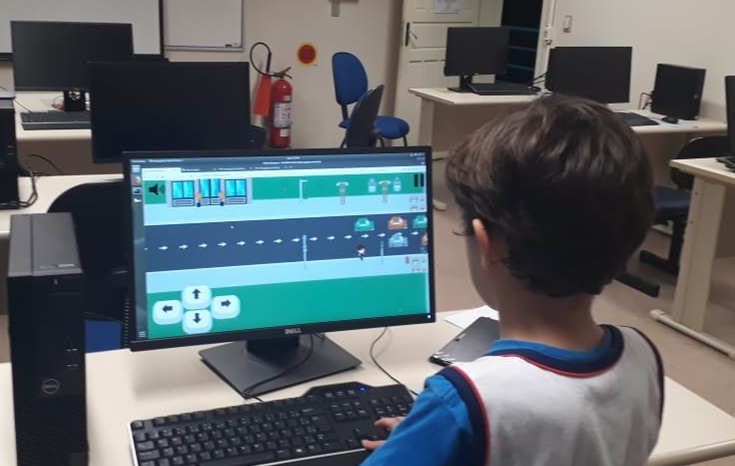
\includegraphics[scale = 0.4]{Figuras/MeninoJogando.png}
    \end{figure}

\end{frame}
%[Transparência 3] Bom, para contextualizar, antes de explicar o artigo relacionado com meu trabalho de mestrado, eu necessito antes, explicar sobre o que é meu trabalho de mestrado.
%Meu trabalho de mestrado é orientado pela doutora Carla, onde nós visamos a prevenção da violência sexual infantil, por meio da utilização de um jogo sério (em outras palavras, um jogo educacional)
%vide isso, existem duas classes de artigos relacionados com meu projeto de mestrado que eu poderia buscar: os artigos focados no jogo em seus jogos em si, e os artigos focados em seus jogadores. Nesse sentido, eu optei pela segunda classe. 


\begin{frame}{ARTIGO RELACIONADO}

    \begin{figure}
        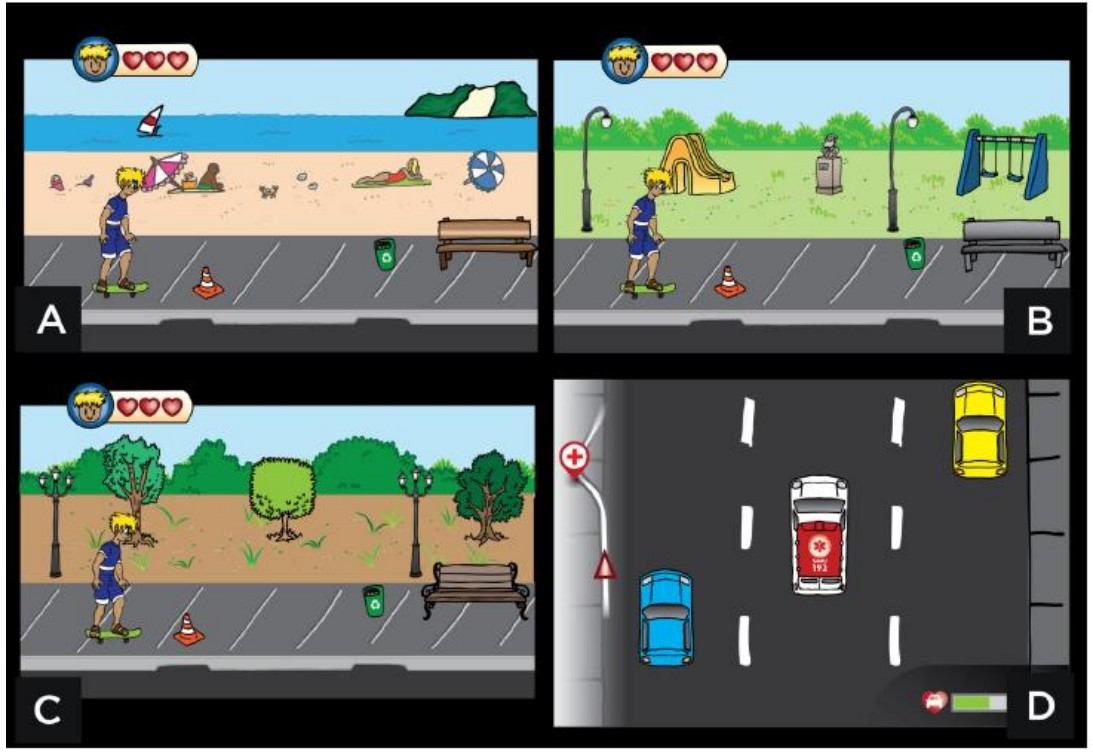
\includegraphics[scale = 0.3]{Figuras/Esquadrao192.jpg}
    \end{figure}

\end{frame}
%[Transparência 4] O Artigo em si, menciona três jogos: Esquadrão 192, Ran-gO e Chico na ilha dos jurubebas.
%Esse aqui no caso é o Esquadrão 192, o qual é um jogo destinado a educar as crianças acerca dos sintomas e procedimentos de emergência do Acidente Vascular Cerebral (AVC).


\begin{frame}{ARTIGO RELACIONADO}
    
    \begin{figure}
        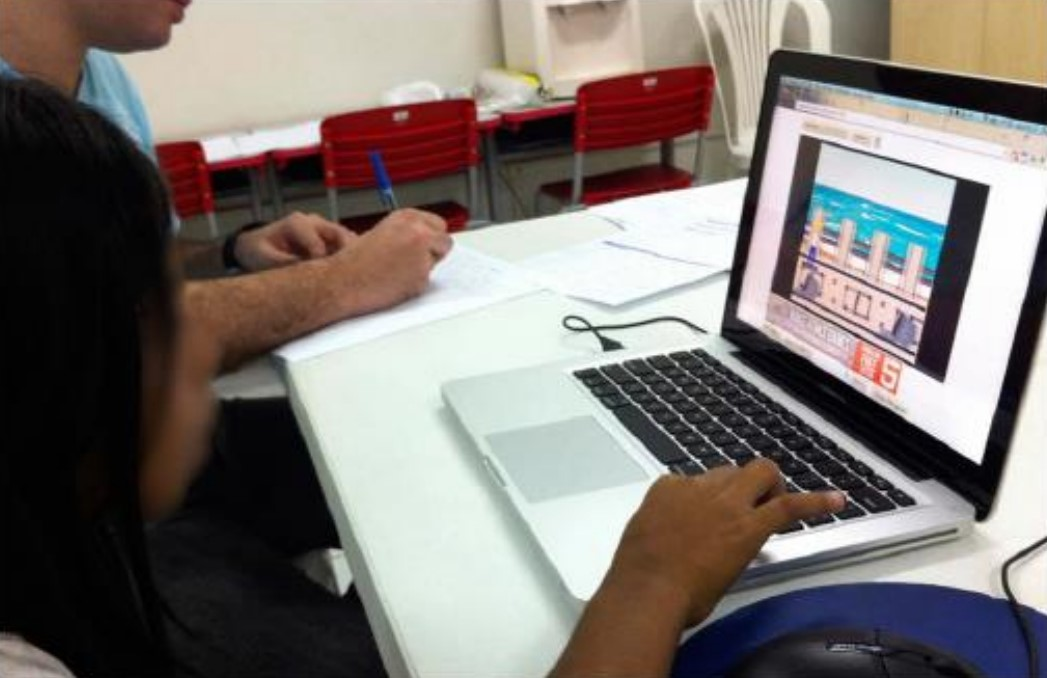
\includegraphics[scale = 0.3]{Figuras/crianca192.jpg}
    \end{figure}

\end{frame}
%[Transparência 5] No entanto, eu não pretendo me focar no jogo em si. Mas sim, na avaliação e nos métodos de análise educacional que eles usaram para medir o conhecimento infantil adquirido. 


\begin{frame}{FLUXO DAS ETAPAS DE AVALIAÇÃO}
    
    \begin{figure}
        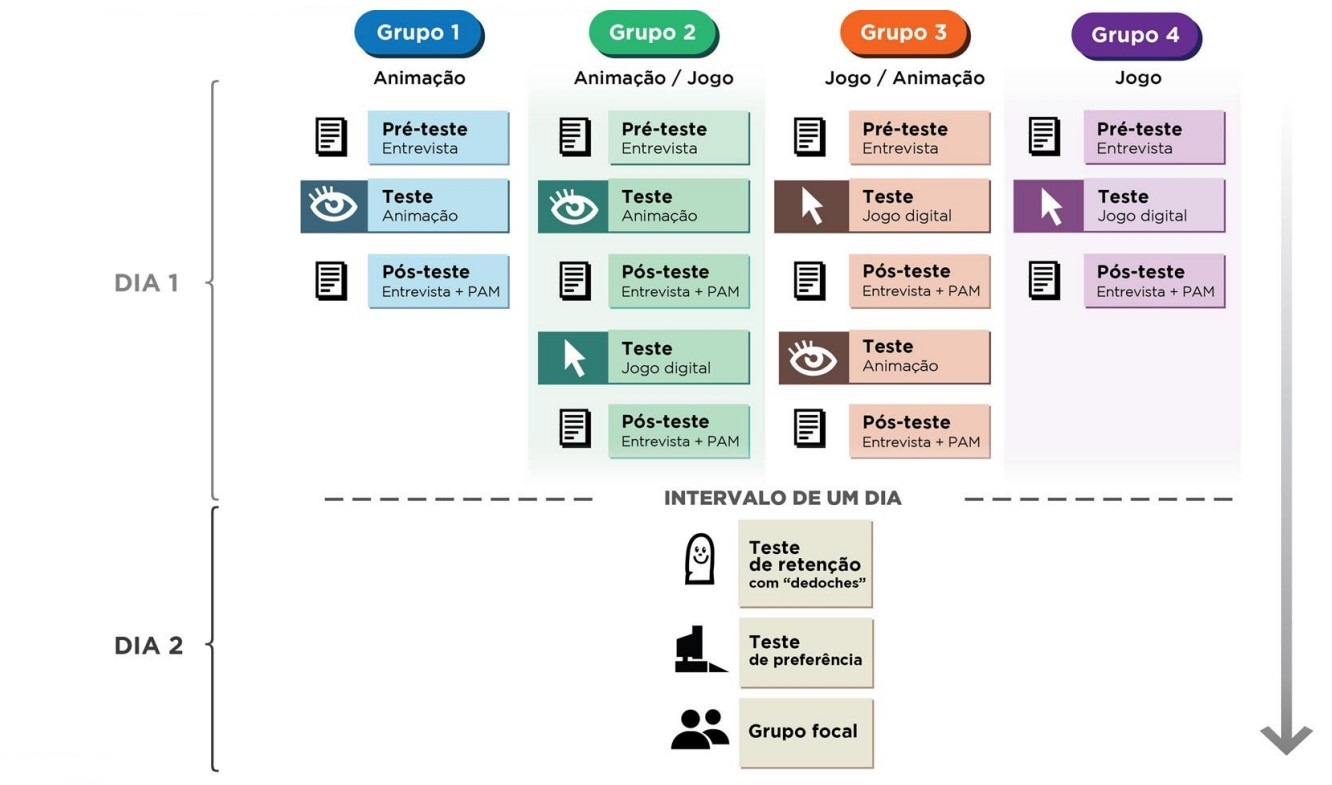
\includegraphics[scale = 0.29]{Figuras/Fluxograma.jpg}
    \end{figure}

\end{frame}
%[Transparência 6] Ao todo participaram 39 crianças, com idades entre 8 e 13 anos. Uma faixa etária bastante próxima do meu projeto de mestrado (5 e 6 anos). Além disso, o jogo também foi construido em Construct 2.
%As crianças foram divididas em 4 grupos. Cabe mencionar aqui, que um dos objetivos da pesquisa era mensurar as diferenças de retenção de informação e de engajamento entre uma animação e um jogo, ambos sobre o mesmo tema. Por tal razão existem 4 grupos, cada qual medindo cada possibilidade entre jogo e animação.


\begin{frame}{PRÉ-TESTE}
    
    \begin{figure}
        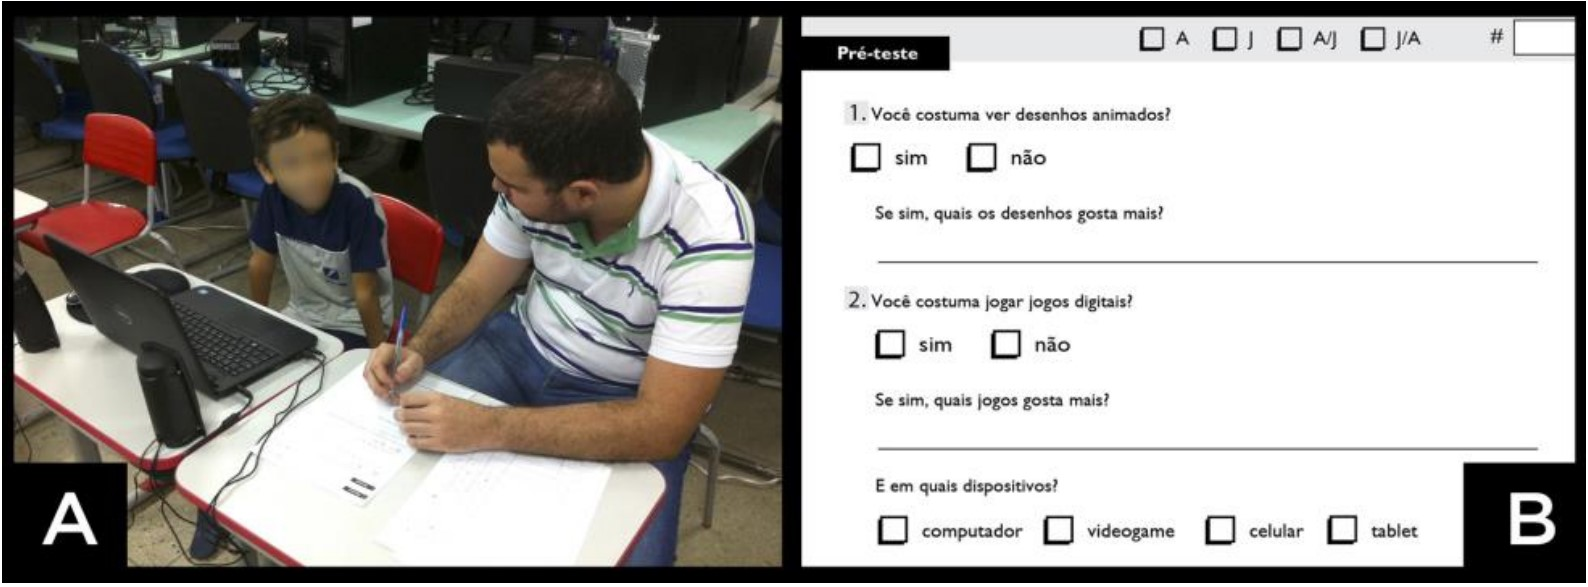
\includegraphics[scale = 0.25]{Figuras/pre-teste.jpg}
    \end{figure}

\end{frame}
%[Transparência 7] No pré-teste, as crianças foram entrevistas de modo a responder determinadas perguntas de forma oral. Além das perguntas aqui visíveis, as crianças eram questionadas sobre seu conhecimento sobre o AVC.


\begin{frame}{TESTE}
    
    \begin{figure}
        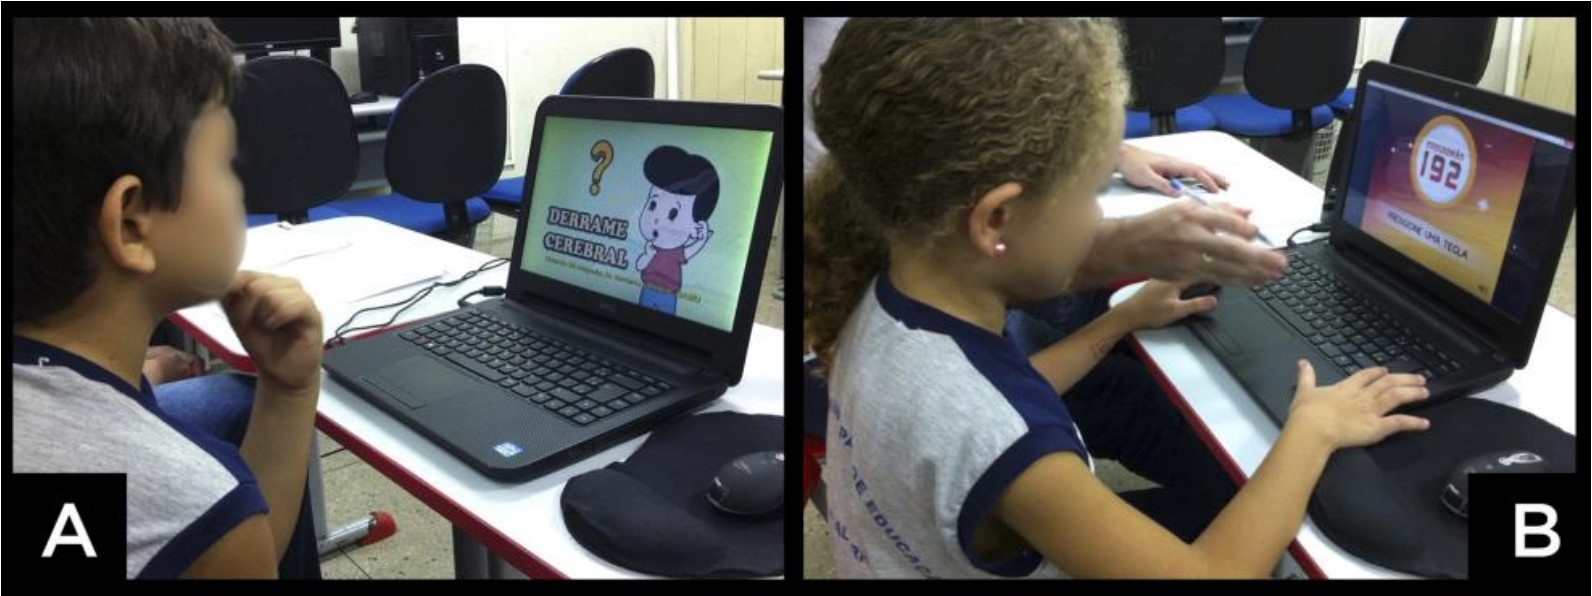
\includegraphics[scale = 0.25]{Figuras/JogoxAnimacao.jpg}
    \end{figure}

\end{frame}
%[Transparência 8] Aqui nós temos dois tipos de testes. À esquerda é possível ver uma criança sendo submetida a animação e à esquerda é possível ver uma criança sendo submetida ao jogo.


\begin{frame}{PÓS-TESTE}
    
    \begin{figure}
        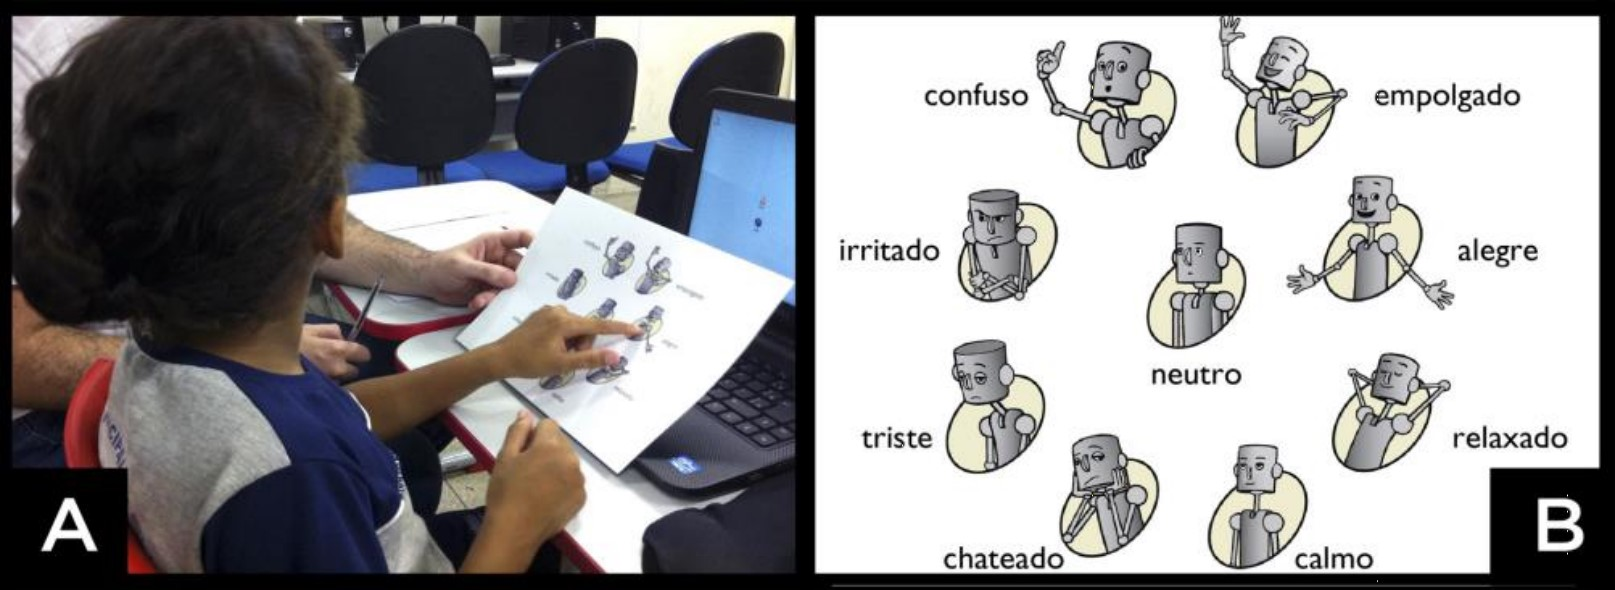
\includegraphics[scale = 0.25]{Figuras/pos-teste.jpg}
    \end{figure}

\end{frame}
%[Transparência 9] No pós-teste as crianças foram submetidas a escala PAM para mensurar seu humor. Além disso, perguntas sobre o número do SAMU, sintomas do AVC, também foram feitas. Para os grupos 2 e 3, foi perguntado qual mídia foi a favorita da criança: o jogo ou a animação. 


\begin{frame}{DEDOCHES}
    
    \begin{figure}
        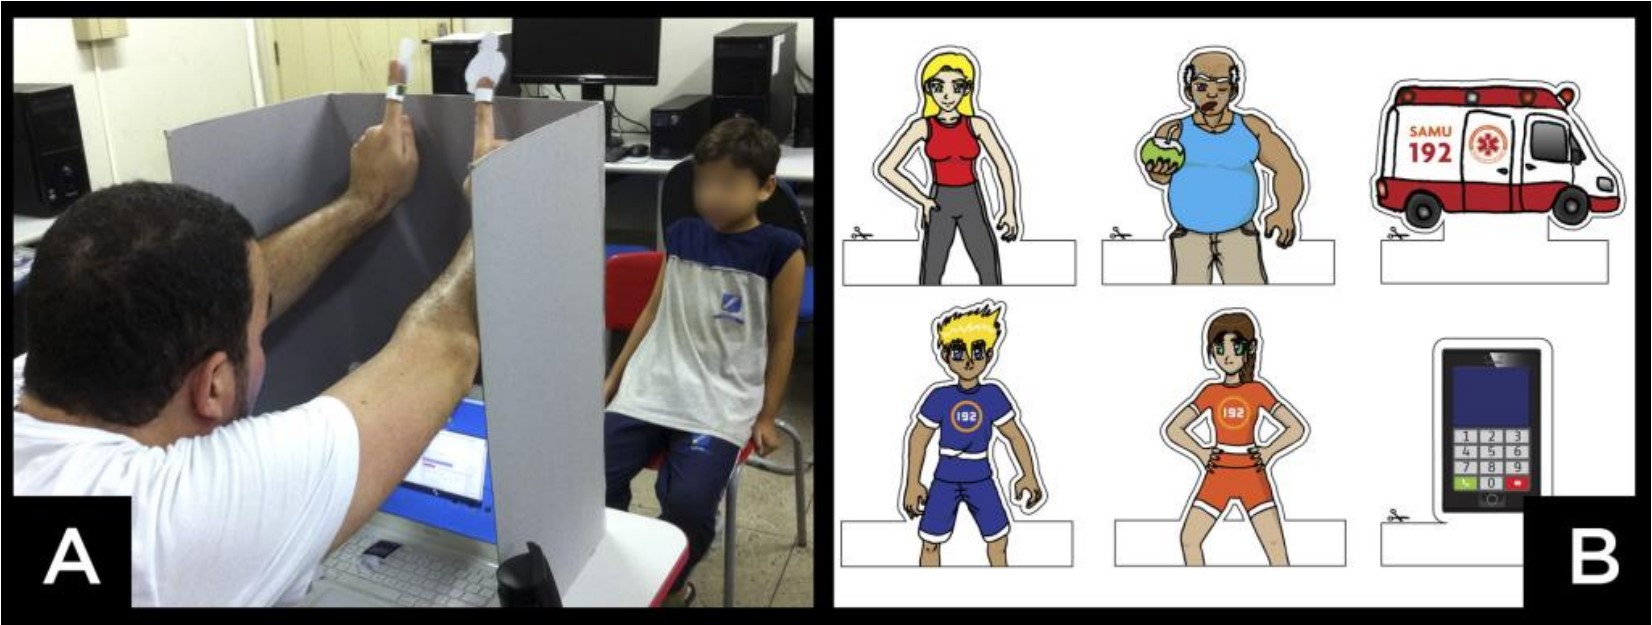
\includegraphics[scale = 0.25]{Figuras/Dedoches.jpg}
    \end{figure}

\end{frame}
%[Transparência 10] Um dia depois, para medir o nível de retenção do conhecimento foi realizado um teatro de bonecos, onde as crianças poderia interagir com os fantoches de modo a manifestar o conhecimento adquirido.


\begin{frame}{TESTE DE PREFERÊNCIA}
    
    \begin{figure}
        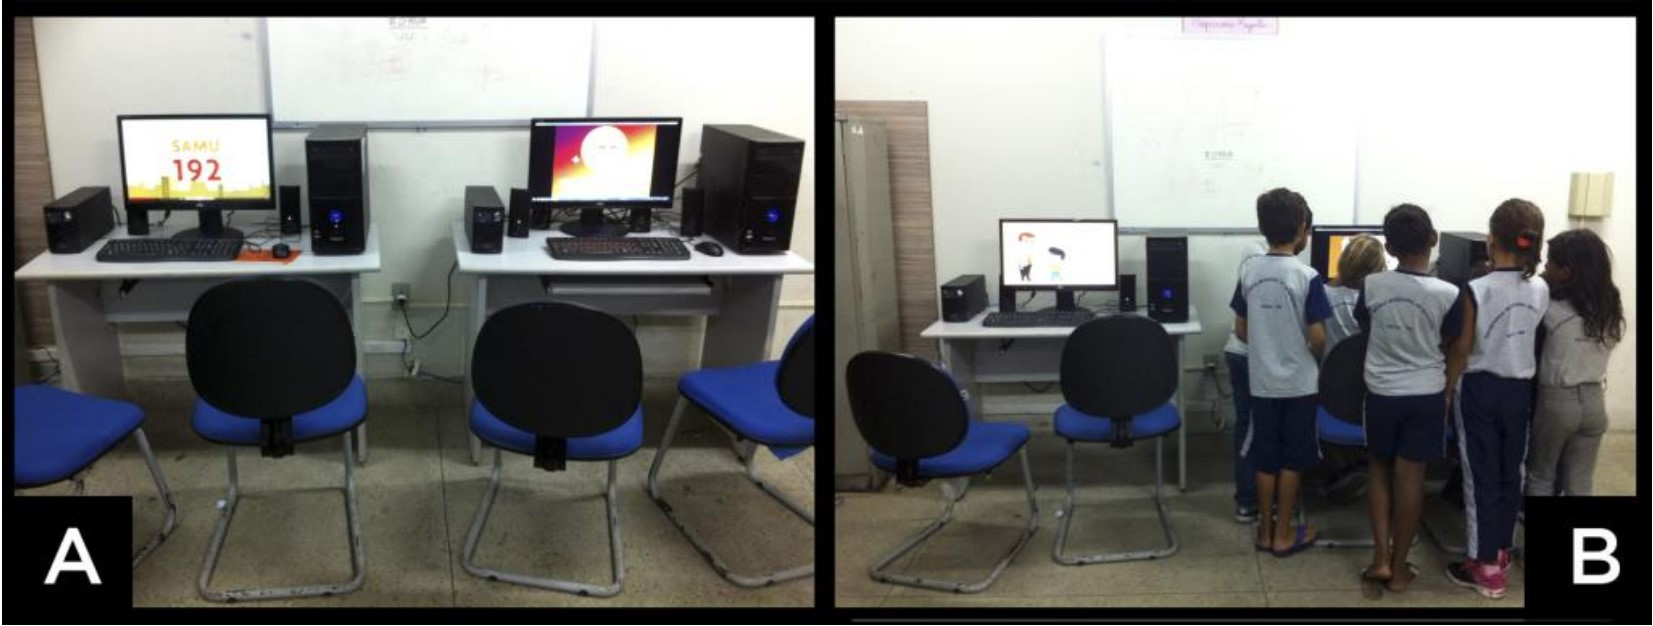
\includegraphics[scale = 0.25]{Figuras/Preferencia.jpg}
    \end{figure}

\end{frame}
%[Transparência 11] O teste de preferência foi realizado por aproximadamente 10 minutos, onde as crianças tinham a sua disposição dois computadores, um munido do jogo e outro da animação. Nesse teste, buscava-se medir o comportamento das crianças nesse cenário.


\begin{frame}{GRUPO FOCAL}
    
    \begin{figure}
        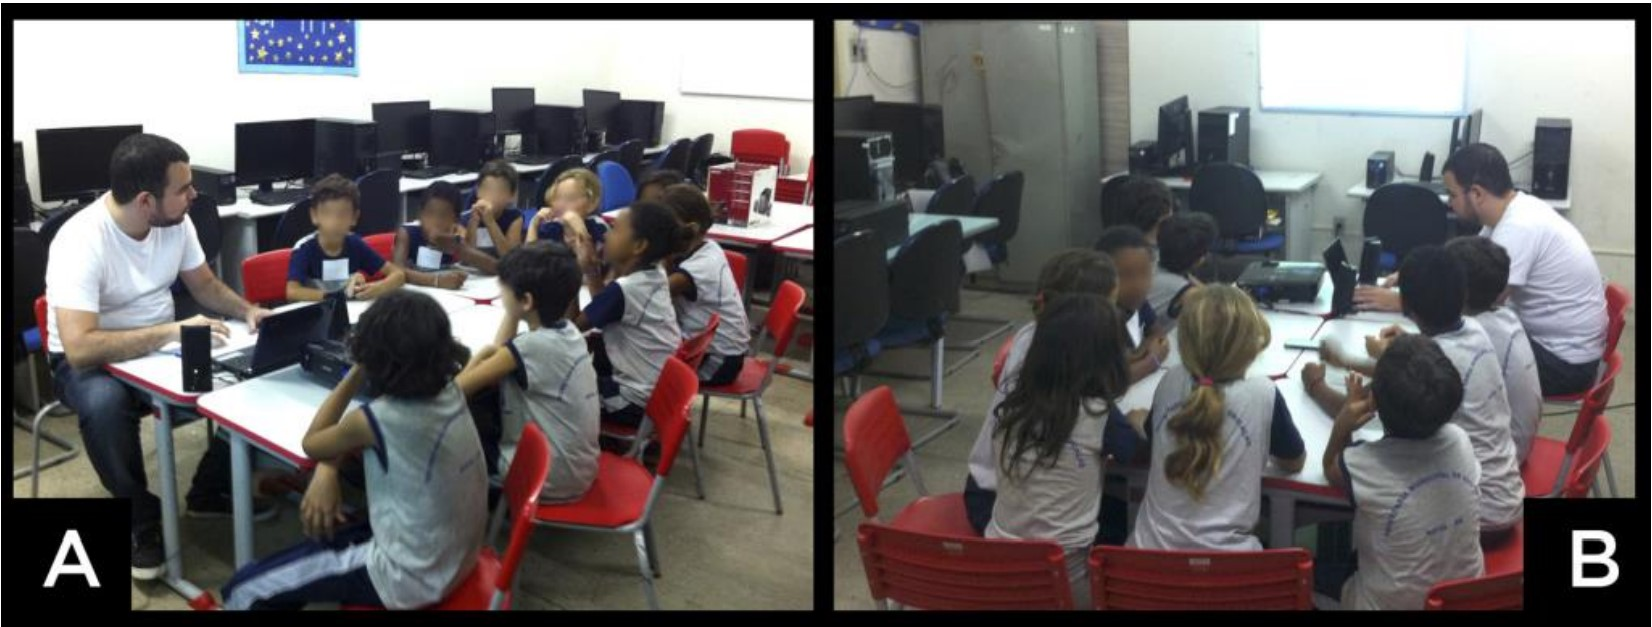
\includegraphics[scale = 0.25]{Figuras/GrupoFocal.jpg}
    \end{figure}

\end{frame}
%[Transparência 12] Por fim foi realizado o grupo focal para extrair opnião de forma coletiva das crianças. 
%Além das crianças poderem se manifestar livremente nessa etapa, foram realizandas algumas perguntas:
%Qual dos dois foi mais interessante? Por quê?
%O que o desenho tem de legal? 
%O que o jogo tem de legal?
%Os personagens são bonitos? 
%A música do jogo é legal?
%Como o jogo poderia ser melhorado? 
%Se pudéssemos inventar outro jogo como seria?


\begin{frame}{CONCLUSÃO}
    
    \begin{figure}
        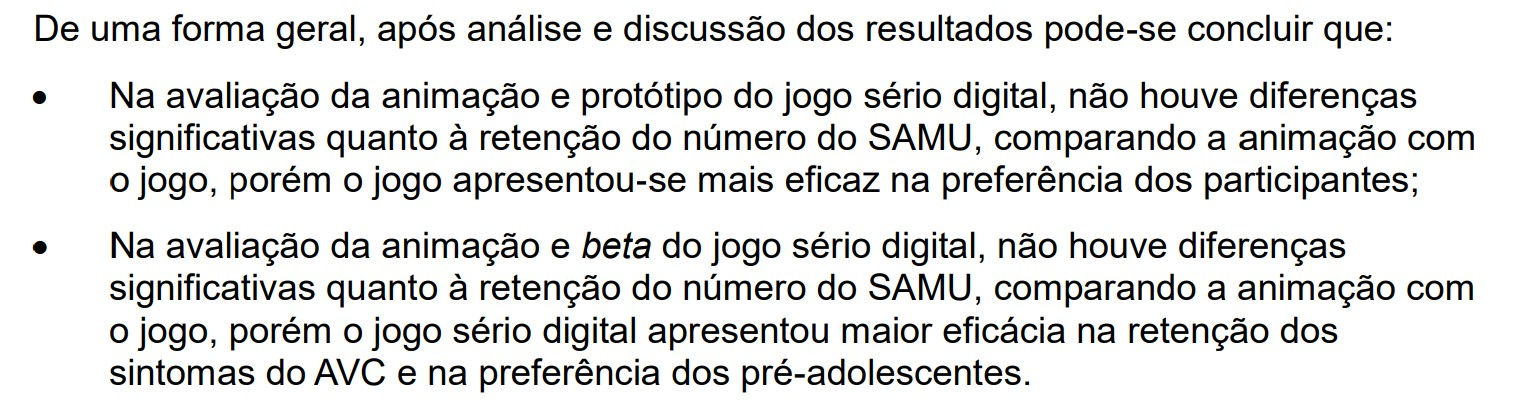
\includegraphics[scale = 0.29]{Figuras/Conclusao.jpg}
    \end{figure}

\end{frame}
%[Transparência 13] Como conclusão geral, o presente artigo notou uma maior fixação do conhecimento por parte das crianças que jogaram o jogo. Somado a isso, o jogo também manifestou ter um maior engajamento.
% Como melhoria, os autores notaram a necessidade da dublagem associada ao texto escrito por causa das dificuldades de leitura e interpretação pelos participantes. No mais, os autores também notaram dificuldades das crianças em alternar entre os perifêricos mouse e teclado.


\begin{frame}
    \begin{center}
        \textit{"Eu não acho que seja justo desprezar qualquer forma de mídia ou entretenimento. Tudo depende de como é feito" - Stan Lee}\\
        \vspace{1.5cm}
        \begin{Huge} 
            Obrigado!\\
        \end{Huge}
        \bigskip
        Alexandre Mendonça Fava - \alert{alexandre.fava@hotmail.com}\\
    \end{center}
\end{frame}

\end{document}